% !TEX root = ../26_11c-all-en-amb-master-ok.tex

\chapter{CENNI DI GEOMETRIA SOLARE}
\label{chp:geometria-solare}

\section{La terra e il sole}
\label{sec:terra-sole}

Il sole fornisce \emph{energia} a tutti i pianeti del suo sistema. L'energia prodotta all'interno del nucleo – ove si raggiunge la temperatura di 14 milioni di gradi Celsius – attraverso reazioni di fusione nucleare raggiunge la terra, la riscalda e fornisce la luce naturale. 

\begin{figure}[ht]
\centering  % ordine per clip: left, lower right upper
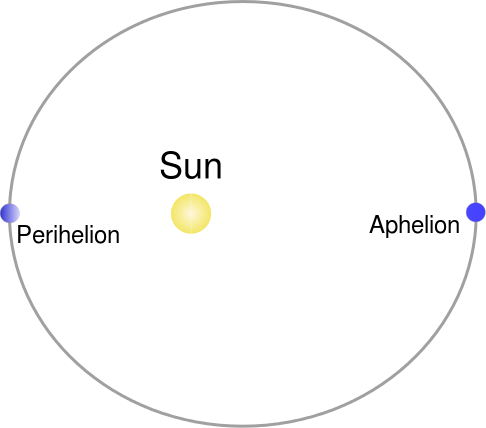
\includegraphics[width=0.4\textwidth,keepaspectratio]{images/wikipedia/Perihelion-Aphelion}
\caption[Orbita-Perielio-Afelio]{Orbita ellittica della terra attorno al sole. Si notano la posizione del sole (Sun) che non coincide con il centro dell'ellisse e le due posizioni di massima (Perihelion) e minima (Aphelion) distanza della terra dal sole. (Fonte: Wikipedia)}
\label{fig:orbita-perielio-afelio}
\end{figure}
La terra ruota attorno al sole (movimento di \emph{rivoluzione}) percorrendo un'orbita ellittica\footnote{La rivoluzione completa attorno al sole si compie in 365,25 giorni. L'eccentricità dell'ellisse è relativamente piccola e l'orbita spesso è approssimata al cerchio (vedi \fref{fig:orbita-perielio-afelio}. Il momento in cui la terra è più vicino al sole, a circa 147 milioni di km (\emph{perielio} o \emph{perihelion}) avviene il 2 di gennaio mentre il 3 luglio è il giorno in cui è più lontana, a circa 152 milioni di km (\emph{afelio} o \emph{aphelion}).} compie un giro completo che vede il sole in posizione decentrata rispetto al suo centro geometrico. Contemporaneamente la terra ruota attorno al proprio asse\footnote{In circa 24 ore compie un giro completo} (movimento di \emph{rotazione}) – che non è verticale ma inclinato di circa \ang{23,45}. Questa inclinazione è all'origine dell'alternanza delle stagioni tra i due emisferi nord e sud poiché ricevono la radiazione solare con angoli differenti: il 21 Giugno\footnote{Solstizio d'estate per l'emisfero nord e viceversa per quello sud. I raggi solari sono perpendicolari al suolo terrestre in corrispondenza del \emph{Tropico del Cancro} (latitudine di \ang{45}).} il polo Nord punta verso il sole, mentre il 21 Dicembre\footnote{Solstizio d'inverno per l'emisfero nord e viceversa per quello sud. I raggi solari sono perpendicolari\footnote{Questa situazione avviene alle ore 12 (solari) e si definisce comunemente con l'espressione: di \emph{sole allo zenit}} al suolo terrestre in corrispondenza del \emph{Tropico del Capricorno} (latitudine di~\ang{-45}).} punta verso il sole il polo Sud. In concomitanza con gli equinozi\footnote{Il 21 Marzo e 21 Settembre. In questi due giorni il centro del sole e della terra possono essere uniti idealmente tramite una linea che passa per l'equatore terrestre: ovunque, sulla terra, si avranno 12 ore di luce e 12 ore di notte, da qui il termine \emph{equinozio}, derivato dal latino che significa \emph{giorno uguale alla notte}. Va ricordato che il \emph{21esimo} giorno del mese, per solstizi ed equinozi, rappresenta una convenzione comune poiché il giorno reale, astronomico, può variare leggermente di anno in anno.} il \emph{il sole è allo zenit} alle ore 12 (solari) solo all'equatore. 

All'inclinazione dell'asse terrestre si deve quindi la definizione di un angolo (verticale) necessario per individuare la posizione del sole rispetto ad un punto qualsiasi della terra: l'angolo zenitale altrimenti definito come \emph{altitudine} solare. Si tratta cioè dell'angolo formato tra:

\begin{itemize}
\item  la retta congiungente il centro del sole ed il punto della terra in esame,
\item la proiezione di tale retta sul piano dell'orizzonte passante per il punto terrestre in questione.
\end{itemize}
 
L'effetto di questa inclinazione determina l'angolo di incidenza della radiazione solare rispetto all'atmosfera\footnote{Conseguentemente definisce anche l'angolo di incidenza al suolo terrestre.} nei diversi punti dell'orbita e di conseguenza la relativa quantità di energia che riesce ad attraversarla per raggiungere il suolo. È infatti evidente che più l'angolo di incidenza tende ad essere verticale, minore sarà la sua riflessione e quindi maggiore la percentuale di energia che potrà penetrare. Ecco perché \emph{in estate}, nonostante l'orbita terrestre ponga il nostro pianeta ad una distanza maggiore dal sole rispetto all'inverno,\footnote{Circa tre milioni di di miglia in più al 21 Giugno.} la temperatura sulla terra è maggiore: il sole è più alto sull'orizzonte, l'angolo di incidenza cresce così come la quantità di radiazione che perfora l'atmosfera e le giornate sono più lunghe.

\begin{table}[htp]
\centering
\caption{Per semplificare i calcoli e facilitare il progettista con applicazioni specifiche la tabella indica il numero di progressivo del primo giorno di ogni mese.}
\label{tab:num-primo-giorno-mese}
\begin{tabular}{@{}lclc@{}}
\toprule
\textit{mese} & \textit{num.} & \textit{mese} & \textit{num.} \\ \toprule
Gennaio       & 1             & Luglio        & 182           \\ %\midrule
Febbraio      & 32            & Agosto        & 213           \\ %\midrule
Marzo         & 60            & Settembre     & 244           \\ %\midrule
Aprile        & 91            & Ottobre       & 274           \\ %\midrule
Maggio       & 121           & Novembre      & 305           \\ %\midrule
Giugno        & 152           & Dicembre      & 335           \\ \bottomrule
\end{tabular}
\end{table}






\section{Le carte solari}
\label{sec:nota-import}

\subsection{Cosa sono}
\label{subsec:cosa-sono}


\subsection{A cosa servono}
\label{subsec:a-cosa-servono}


\subsection{Come si usano}
\label{subsec:come-si-usano}

\subsection{Carte di base per Casal Cermelli}
\label{subsec:carte-base}